

\section{Modellazione RTL}

La prima versione del cifratore (RTL) viene implementata a partire dal sorgente fornito. Il primo compito svolto è stato schematizzare il codice in un diagramma di flusso (Figura~\ref{fig:algo}). 

\begin{figure*}[htbp]
    \centering
    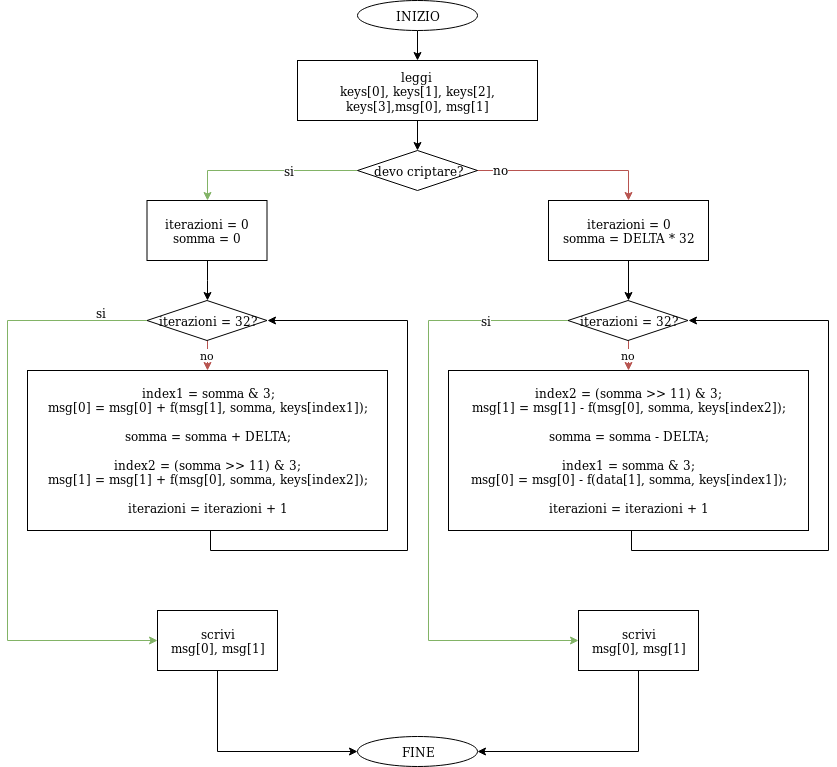
\includegraphics[width=0.7\textwidth]{schemi/algo.png}
    \caption{Algoritmo ad alto livello del cifratore. NB: La funzione $f(a,b,c)$ è un'espressione che corrisponde a $(((a \ll 4) \oplus (a \gg 5)) + a) \oplus (b + c)$.}
    \label{fig:algo}
\end{figure*}

Questo permette di estrarre gli input e gli output che servono al modulo per funzionare. Una prima soluzione potrebbe essere prende in input tutti i dati che servono in una volta sola: la chiave, i dati da elaborare, la modalità di esecuzione.

In realtà l'interfaccia risulta grossolana: il cifratore probabilmente dovrà elaborare un discreto numero di dati utilizzando sempre la stessa chiave (intesa come il gruppo di 128 bit). Risulta inutile passarla sempre quando per la maggior parte delle computazioni questa rimarrà identica. Si sceglie quindi di togliere l'input relativo alla chiave. Questa verrà passata all'inizio della computazione utilizzando la porta \code{data}. Poiché la porta \code{data} è di 64bit e la chiave è grande il doppio, occorrerà passarla in due volte. Otteniamo lo schema che segue:
\begin{center}
    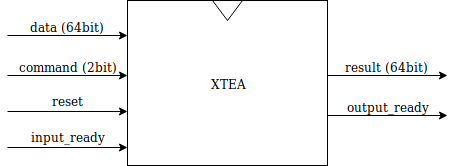
\includegraphics[width=0.35\textwidth]{schemi/rtl_interface.png}
\end{center}

Le porte hanno il seguente significato:
\begin{itemize}
    \item \code{clock} (in input);
    \item \code{reset} (in input): quando attivo alto, riporta il modulo allo stato iniziale;
    \item \code{command} (in input, 2bit): comando da eseguire sul modulo;
    \item \code{data} (in input, 64bit): valore da processare;
    \item \code{input\_ready} (in input): quando attivo alto, si possono leggere i dati in input;
    \item \code{result} (in output, 64bit): risultato della computazione;
    \item \code{output\_ready} (in output): quando è attivo alto, la computazione è terminata;
\end{itemize}

L'azione corrispondente ai valori forniti in input è presente in Tabella~\ref{tab:azioni}. Una volta che il modulo ha finito la computazione, viene attivato il segnale \code{output\_ready} e viene mantenuto attivo un solo ciclo di clock. Durante questo periodo di tempo si può leggere il valore della porta \code{result}.

\begin{table*}[htbp]
    \centering
    \begin{tabular}{lllp{5cm}}
        \toprule
        reset & input\_ready & command & azione \\ \cmidrule{1-4}
         \code{1} & \code{-} & \code{--} &	riporta il sistema allo stato iniziale
        \\ \code{0} & \code{0} & \code{--} &	non fare nulla
        \\ \code{0} & \code{1} & \code{00} &	memorizza il valore su data all’interno del sistema come i primi 64bit della chiave
        \\ \code{0} & \code{1} & \code{01} &	memorizza il valore su data all’interno del sistema come i secondi 64bit della chiave
        \\ \code{0} & \code{1} & \code{10} &	avvia la criptazione, il messaggio è il valore su data
        \\ \code{0} & \code{1} & \code{11} &	avvia la decriptazione, il messaggio è il valore su data \\ \bottomrule
    \end{tabular}
    \caption{Tabella delle azioni}
    \label{tab:azioni}
\end{table*}

Si è deciso di dividere il modulo in due funzioni separate: una funzione è \code{fsm} e l'altra \code{datapath}. La prima ha il compito di leggere i dati in input e memorizzarli all'interno del modulo, scandire l'avanzamento della computazione modificando la variabile di stato, e scrivere i valori in output. La seconda si occupa di elaborare espressioni aritmetiche anche semplici. 

Si può notare nell'algoritmo in Figura~\ref{fig:algo} che buona parte dei due blocchi più grandi, quelli contenenti i calcoli, si sovrappone. Per questo il modulo cercherà di sfruttare quando può questa sovrapposizione per minimizzare l'area (del datapath, nella quale vengono effettuate queste computazioni). 

Inoltre le operazioni $\text{index} = x \text{\&} 3, \; \text{index} = (x \gg 11) \text{\&} 3$ usate per calcolare quale parte di chiave si traducono in una semplice estrazione di bit dall'operando, quindi non serve passare dal datapath.

Il compito della FSM è legge gli input e li salva all'interno delle propri registri, gestisce lo stato, comunica col datapath e scrive gli output. Il datapath legge i dati dai registri della FSM e li sposta nei propri registri effettua le operazioni aritmetiche. In Figura~\ref{fig:internal} puoi vedere la mappa dei registri. Ogni registro è scritto o solo dalla FSM o solo dal datapath.

\begin{figure}[htbp]
    \centering
    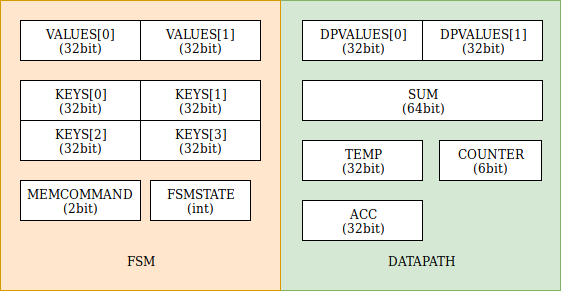
\includegraphics[width=0.45\textwidth]{schemi/rtl_registers.png}
    \caption{Registri interni al modulo}
    \label{fig:internal}
\end{figure}

Lo schema compatto di FSM e datapath è presente sottoforma di schema in Figura~\ref{fig:efsm}. I cerchi sono gli stati, le etichette sulle freccie indicano la condizione con la quale viene cambiato lo stato. In rettangoli verdi sono i calcoli svolti dal datapath. Come si può notare, le operazioni fatte in alcuni stati sono uguali, il che ci permette di ottimizzare per area il nostro modulo. 

\begin{figure*}[htbp]
    \centering
    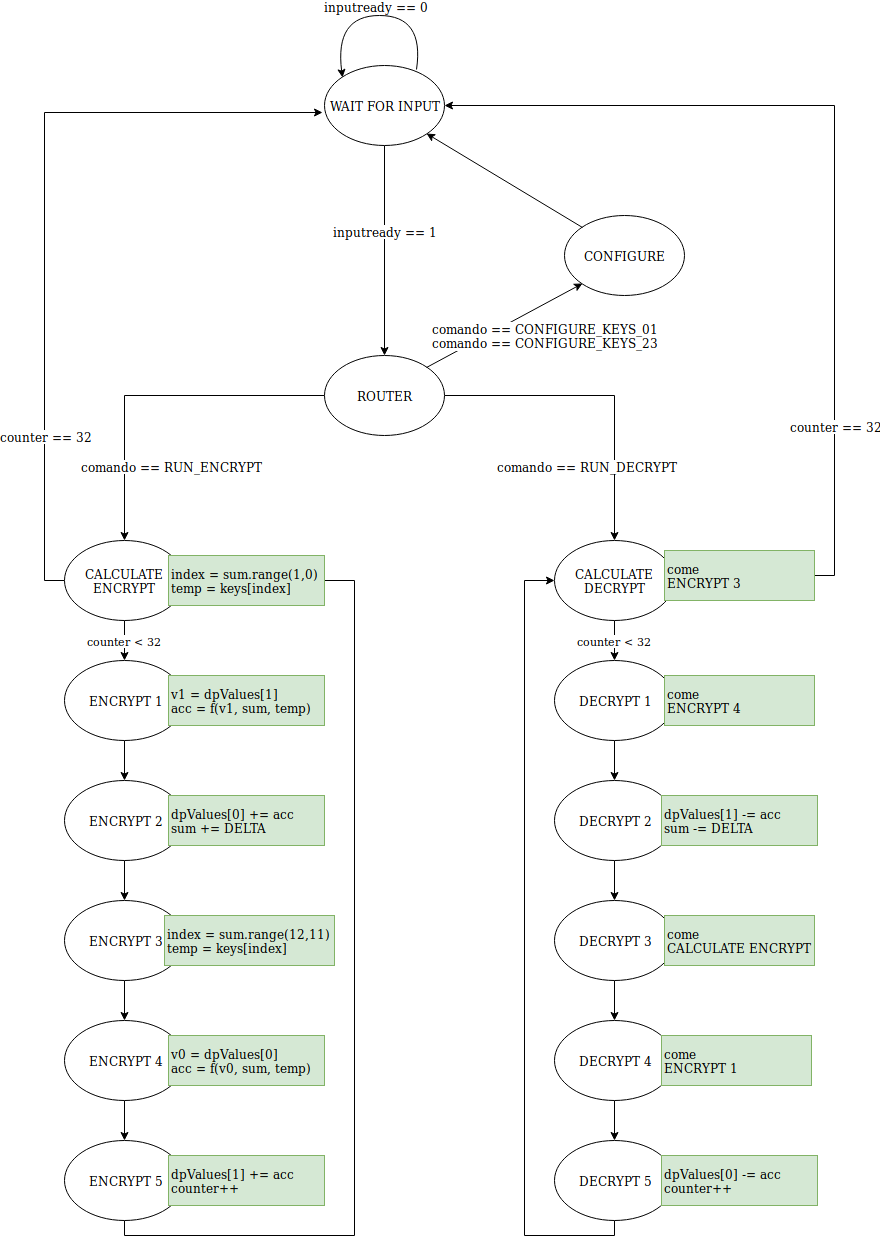
\includegraphics[width=0.7\textwidth]{schemi/rtl_efsm.png}
    \caption{Diagramma degli stati. Le transazioni sono comandate dalla FSM. In verde sono presenti le elaborazioni fatte dal datapath}
    \label{fig:efsm}
\end{figure*}